
%!TEX root = ./main.tex



\tikzset{every picture/.style={line width=0.75pt}} %set default line width to 0.75pt        

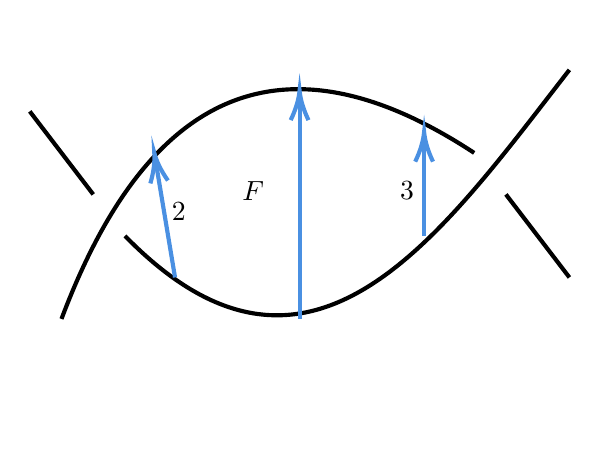
\begin{tikzpicture}[x=0.75pt,y=0.75pt,yscale=-1,xscale=1]
%uncomment if require: \path (0,877); %set diagram left start at 0, and has height of 877

%Curve Lines [id:da19609189587014564] 
\draw [line width=1.5]    (195.29,140) .. controls (237.61,27.33) and (303.88,0.67) .. (394.12,60) ;
%Straight Lines [id:da2771116463618114] 
\draw [line width=1.5]    (180,40) -- (210.59,80) ;
%Curve Lines [id:da5075059974941536] 
\draw [line width=1.5]    (225.88,100) .. controls (315.1,191.33) and (377.29,100.67) .. (440,20) ;
%Straight Lines [id:da01404980269438516] 
\draw [line width=1.5]    (409.41,80) -- (440,120) ;
%Straight Lines [id:da6027225475778994] 
\draw [color={rgb, 255:red, 74; green, 144; blue, 226 }  ,draw opacity=1 ][line width=1.5]    (250,120) -- (240.49,62.96) ;
\draw [shift={(240,60)}, rotate = 80.54] [color={rgb, 255:red, 74; green, 144; blue, 226 }  ,draw opacity=1 ][line width=1.5]    (14.21,-4.28) .. controls (9.04,-1.82) and (4.3,-0.39) .. (0,0) .. controls (4.3,0.39) and (9.04,1.82) .. (14.21,4.28)   ;
%Straight Lines [id:da602091940582576] 
\draw [color={rgb, 255:red, 74; green, 144; blue, 226 }  ,draw opacity=1 ][line width=1.5]    (370,100) -- (370,53) ;
\draw [shift={(370,50)}, rotate = 90] [color={rgb, 255:red, 74; green, 144; blue, 226 }  ,draw opacity=1 ][line width=1.5]    (14.21,-4.28) .. controls (9.04,-1.82) and (4.3,-0.39) .. (0,0) .. controls (4.3,0.39) and (9.04,1.82) .. (14.21,4.28)   ;
%Straight Lines [id:da7589682295521507] 
\draw [color={rgb, 255:red, 74; green, 144; blue, 226 }  ,draw opacity=1 ][line width=1.5]    (310,140) -- (310,33) ;
\draw [shift={(310,30)}, rotate = 90] [color={rgb, 255:red, 74; green, 144; blue, 226 }  ,draw opacity=1 ][line width=1.5]    (14.21,-4.28) .. controls (9.04,-1.82) and (4.3,-0.39) .. (0,0) .. controls (4.3,0.39) and (9.04,1.82) .. (14.21,4.28)   ;

% Text Node
\draw (281,72.4) node [anchor=north west][inner sep=0.75pt]    {$F$};
% Text Node
\draw (247,82.4) node [anchor=north west][inner sep=0.75pt]    {$2$};
% Text Node
\draw (357,72.4) node [anchor=north west][inner sep=0.75pt]    {$3$};


\end{tikzpicture}